Classical cryptography can be divided into several fields of study, two of which are of particular interest to us: 
symmetric-key and public-key cryptography. 
The former, and oldest of the two, involves both, Alice and Bob, sharing a common key,
\begin{figure}[!h]
\centerline{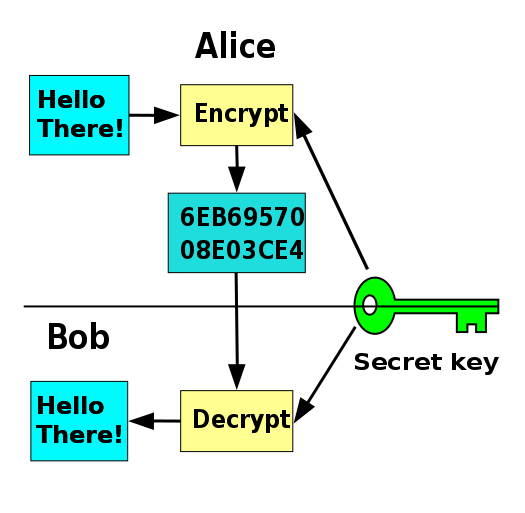
\includegraphics[width=\textwidth,height=\textheight,keepaspectratio]{1.png}}
\caption{A popular symmetric-key encryption method: Advanced Encryption Standard (AES).}
\label{fig1}
\end{figure}
while, the latter involves using a pair of keys: public and private, where anyone holding the public key
can encrypt the data bits, but which only the holder of the private key can decrypt.
\begin{figure}[!h]
\centerline{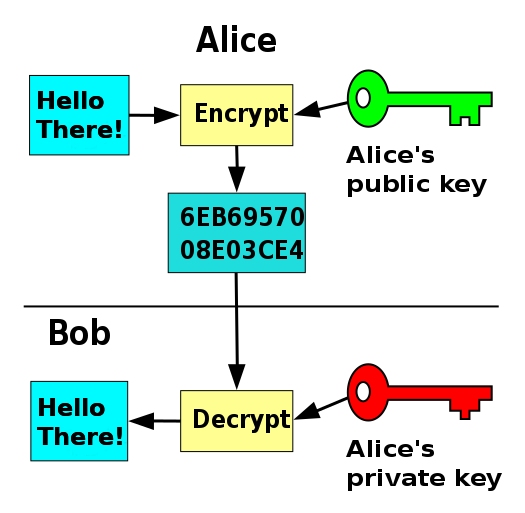
\includegraphics[width=\textwidth,height=\textheight,keepaspectratio]{2.png}}
\caption{Popular examples of public-key encryption: RSA (Rivest-Shamir-Adleman) 
and Elliptic-curve cryptography (ECC).}
\label{fig2}
\end{figure}
And thus, the security wholly depends on the secrecy of the private key.

Before reviewing QKD, we will take a look at some examples of encrypting and decrypting data.
We will assume two parties, Alice and Bob, who want to share a private message over an public channel. 
Using a trivial method we generate a random integer key $k$ to which we can then 
add each message character in order to encrypt it.
Let's represent the capital letters of the alphabet using binary encoding:\\
\centerline{$2^{\bm{4}}=16<(\#\ letters\ in\ alphabet)=26<2^{5}=32 \rightarrow (\#\ encoding\ bits) = \bm{5}$:}\\
\centerline{$\textbf{A} \rightarrow 0000,\ \textbf{B} \rightarrow 0001,\ \textbf{C} \rightarrow 0010,\ \textbf{D} \rightarrow 0011$,\ etc.}\\
But, since the communication channel is public, Eve can easily tap into the line (e.g. optical fiber) 
and steal the data that is being transmitted without the parties realizing it.

So, how can the parties secure the message?
A very simple means of securing the message is to generate an integer key $k$ to add to each character before transmission so that
when Bob receives the message, he need only subtract $k$ from each character to retrieve the original copy. 
That makes it inconvenient for Eve to steal any data without knowing $k$.\\~\\
\textbf{\underline{Example}}:
Alice encrypts message $\textbf{m}$ by adding key $\textbf{k}$ to each of its characters $\textbf{c}$:\\~\\
\centerline{$\textbf{m} = \textbf{c} + \textbf{k}$}\\~\\
Let's say Alice wants to share \textbf{HELLO} with Bob, and $k = 3$ (0011):
\\
\begin{center}
$\textbf{H} \rightarrow 00111 \rightarrow 01010 \rightarrow \textbf{K}$ \\
$\textbf{E} \rightarrow 00100 \rightarrow 00111 \rightarrow \textbf{H}$ \\
$\textbf{L} \rightarrow 01011 \rightarrow 01110 \rightarrow \textbf{O}$ \\
$\textbf{L} \rightarrow 01011 \rightarrow 01110 \rightarrow \textbf{O}$ \\
$\textbf{O} \rightarrow 01110 \rightarrow 10001 \rightarrow \textbf{R}$ \\
\end{center}
~\\
Alice encrypts $\textbf{HELLO} \rightarrow \textbf{KHOOR}$, transmits it over the public channel where Eve might eavesdrop,
but if she does not know the key she will not be able to understand the message. Bob then receives it and decrypts it back 
to the original message $\textbf{KHOOR} \rightarrow \textbf{HELLO}$ by subtracting the shared key $k$:\\~\\
\centerline{$\textbf{m} = \textbf{c} - \textbf{k}$}\\~\\
Of course, the risk of eavesdropping can be minimized by employing a more sophisticated method.
Let's take a look at a more realistic example: RSA, 
which involves four steps: key generation, key distribution, encryption, decryption.\\\\
\textbf{\underline{Example}}:\\
\begin{enumerate}
    \item \textbf{\textit{Key generation}}:
        \begin{itemize}
            \item Choose two distinct prime numbers, such as: $p = 61$, $q = 53$
            \item Compute $n = p \times q = 3233$
            \item Compute the totient of the product $\lambda(n) = lcm(p - 1, q - 1)$:\\
                $\lambda(3233) = lcm(60, 52) = 780$
            \item Choose any number $1 < e < \lambda(n)$ that is coprime to $\lambda(n)$:\\
                  Let's choose $e = 17$
            \item Compute d, where $d \times e \equiv 1 (mod\ \lambda(n))$:\\
                  Let’s choose $d = 413$
        \end{itemize}

    \item \textbf{\textit{Key distribution}}:\\
        Bob publicly transmits his public key $(n, e)$ to Alice (so she can encrypt the message), whereas Bob's private key
        $(n, d)$ (that decrypts the message) is never revealed.
    \item \textbf{\textit{Encryption}}:\\
        The public key is $(n = 3233, e = 17)$, and so for a padded plain-text message $m$, the encryption function is:~\\~\\
        \centerline{$c(m) = (m^e)\ mod\ n = (m^{17})\ mod\ 3233$}
    \item \textbf{\textit{Decryption}}:\\
        The private key is $(n = 3233, d = 413)$. For an encrypted cipher-text $c$, the decryption function is:~\\~\\
        \centerline{$m(c) = (c^d)\ mod\ n = (c^{413})\ mod\ 3233$}\\~\\
        Thus, to encrypt, let’s say, $m = 65$: $c(65) = 2790$\\
        And to decrypt $c = 2790$: $m(2790) = 65$
\end{enumerate}
~\vspace{0.25in}\\
\textbf{\underline{The problem}}: Although it is extremely difficult (very-very slow) for a classical computer to factor a sufficiently 
large enough $n$ into its $p$ and $q$, Shor's algorithm demonstrates that a quantum computer can easily accomplish that task. 
Meaning, that for a quantum system there arises the need for a better-suited cryptographic scheme.
